% chercher des documents LaTeX dans styles, corps et bib
\makeatletter\def\input@path{{styles/}{corps/}{bib/}}\makeatother

% Utiliser le style rapport.cls
\documentclass[12pt, a4paper]{report}

\usepackage[a4paper,vdivide={*,23cm,4cm}]{geometry}
\usepackage[french]{babel} % style francais
\usepackage{styles/pageGardeEnsta}
\usepackage[T1]{fontenc}
\usepackage[utf8]{inputenc} % pour taper les accents directement
\usepackage{lmodern}
\usepackage{amsmath}
\usepackage{amsfonts}
\usepackage{amssymb}

\usepackage{caption}
\usepackage{subcaption}

\usepackage{titlesec}
%\titleformat*{\section}{\fontfamily{lmss}\selectfont\Large\bfseries}
\renewcommand{\thesection}{\Roman{section}.}
\titlespacing*{\section}{0pt}{\baselineskip}{.5\baselineskip}

\titleformat*{\subsection}{\fontfamily{lmss}\selectfont\large\bfseries}
\titlespacing*{\subsection}{1em}{.7\baselineskip}{.5\baselineskip}
\renewcommand{\thesubsection}{\arabic{section}.\arabic{subsection}.}
\renewcommand{\thesubsubsection}{\thesubsection\arabic{subsubsection}}
\titlespacing*{\subsubsection}{0pt}{.5\baselineskip}{.3\baselineskip}

\renewcommand{\labelenumi}{\textbf{\arabic{enumi}.}}


%\usepackage{fourier}

\usepackage[hidelinks]{hyperref}

% chemistry
\usepackage[version=3]{mhchem}

\graphicspath{{imgs/}}
% liens hypertexte dans le document
\usepackage{xcolor}
\usepackage{textcomp}

\usepackage{lastpage}

\usepackage{pgf-umlcd}

\usepackage{fancyhdr}
\pagestyle{fancy}
\fancyhf{}
\fancyhead[L]{}
\fancyhead[C]{}
\fancyhead[R]{Projet d'informatique}
\fancyfoot[L]{}
\fancyfoot[C]{}
\fancyfoot[R]{Page \thepage{} sur~\pageref{LastPage}}

\usepackage{lscape}


\title{Jeu du tarot Africain}
\author{Nicolas \textsc{Dias}\\
  Thomas \textsc{Prévost}}
\date{\today}
\doctype{Projet d'informatique}
\promo{FISE 2024}
\etablissement{\textsc{Ensta} Bretagne\\ 2, rue François Verny\\
   29806 \textsc{Brest} cedex\\ \textsc{France}}
\logoEcole{
\includegraphics[height=4.2cm]{logo_ENSTA_Bretagne_Vertical_CMJN}}


\newcommand{\ie}{\textit{i.e.}}

\begin{document}

\maketitle

   % \section*{Introduction}
  Lorem ipsum dolor sit amet, consectetur adipiscing elit.
  Donec euismod urna eu nisl porttitor, euismod aliquam nunc aliquet.
  Nulla facilisi.
  Etiam euismod, nunc euismod, lacus nunc aliquet, lacus nunc ornare sem, dictum porttitor nisi nisl euismod.

  \vspace{3em}
\begin{center}
  \begin{Large}
* \\
*  \ \ *
\end{Large}
\end{center}





   \tableofcontents

   % \noindent\textit{Le code source complet du projet est disponible sur GitHub :}

\begin{center}
   {\color{blue}\url{https://github.com/thomas40510/ProjetInfoS2}}
\end{center}

\hrulefill


\section{Présentation du projet}\label{sec:présentation-du-projet}
   Nous avons choisi, pour ce projet d'informatique, d'implémenter en Python le jeu du Tarot Africain, qui est un jeu de cartes opposant de deux à quatre joueurs, et demandant stratégie, réflexion mais aussi une part de chance.

   \subsection{Règles du jeu et objectifs du projet}\label{subsec:règles-du-jeu-et-objectifs-du-projet}
      Une partie de Tarot Africain se déroule assez simplement.
      Pour commencer, il faut se munir d'un jeu de tarot, que l'on trie.
      On place alors d'un côté les atouts (du 1 au 21 ainsi que l'excuse) et d'un autre le reste des cartes séparé et trié par couleur\footnote{pique, carreau\dots}.
      \subsubsection{Début de partie}
         Donner, à chaque joueur, un paquet trié de cartes de couleur : elles représentent les vies du joueur et sont placées devant lui, visibles de tous les autres joueurs.
         Les cartes de tarot seront mélangées entre chaque partie.
      \subsubsection{Déroulement d'une partie}
         Au début de chaque manche, un joueur désigné distribue 5 cartes d'atout à chaque joueur.
         Chaque joueur, en commençant par le celui ayant distribué, placera alors un pari sur le nombre de tours qu'il va gagner après avoir consulté ses cartes.
         Chaque joueur est libre de proposer un nombre de son choix, à l'exception du dernier à parler devant proposer un nombre tel que l'ensemble des paris soit différent du nombre de cartes que les joueurs ont en main (5 au premier tour).

         Les joueurs jouent alors à tour de rôle une carte de leur main, en commençant toujours par celui ayant distribué.
         Gagne le tour le joueur ayant placé la carte la plus forte (à noter que le joueur ayant placé l'excuse choisit sa valeur en fonction de sa stratégie : soit elle est la plus forte, soit elle est la plus faible).
         Ce joueur débutera le tour suivant, et ainsi de suite jusqu'à ce qu'il ne reste aucune carte en main.

         En fin de manche, les joueurs perdent autant de vies qu'il leur manque de plis pour remplir leur pari (par exemple, un joueur ayant placé un pari de 3 et n'ayant gagné qu'un pli perd $3-1 = 2$ vies).

         Commence alors la manche suivante, au cours de laquelle seront distribuées 4 cartes (puis 3 à la suivante, puis 2, puis une seule).
      \subsubsection{Tour à une seule carte}
         Le tour à une seule carte est particulier : chaque joueur ne regarde pas sa carte, mais la pose sur son front.
         Il est donc capable de voir uniquement les cartes des autres joueurs et estime s'il est capable de remporter ce pli.

         Là encore, s'applique la même condition sur le dernier joueur à parier (la somme totale ne peut pas être égale à 1).

      \subsubsection{Règle de la \og remontée \fg{}}
         Une règle supplémentaire existe : si, à l'issue d'une manche, un joueur est le seul à ne pas perdre de point, il en regagne un.

      \subsubsection{Fin de partie}
         Une partie se finit à l'issue de la manche d'une seule carte.
         À ce moment là, le jeu peut continuer, chaque joueur gardant le nombre de vies qu'il avait à l'issue de la partie précédente.
         Le joueur ayant distribué transmettant ce rôle à celui à sa gauche.

         Le jeu continue alors de partie en partie jusqu'à ce que tous les joueurs sauf un soient éliminés.

   \subsection{Pistes envisagées pour l'implémentation}\label{subsec:pistes-envisagées-pour-l'implémentation}
      Il a alors été initialement choisi, pour implémenter le jeu de Tarot Africain, le découpage en plusieurs classes : une classe \texttt{Joueur}, une classe \texttt{Carte}, une classe \texttt{Manche} et une classe \texttt{Partie}.
      Structure permettant de manipuler ces différents objets afin de dérouler une partie complète.

      Une première structure du programme a alors été schématisée à partir de ces pistes techniques, soulevant alors plusieurs questions au sein du binôme, impliquant finalement de reconsidérer le découpage qui avait été réalisé initialement.

   \subsection{Choix techniques}\label{subsec:choix-techniques}
      Notre choix, après l'étude préalable ayant été menée, s'est donc porté sur un découpage plus simple que celui initialement prévu : la classe \texttt{Carte}, bien trop simple, n'ayant pas de raison d'exister.

      Le projet s'articule donc, à ce stade, autour de 3 classes principales :
      \begin{itemize}
         \item La classe \texttt{Joueur}, de laquelle sont héritées les classes \texttt{JoueurHumain} et \texttt{JoueurBot} permettant de faire jouer un humain ou la machine ;
         \item La classe \texttt{Manche} permettant de dérouler une manche de la partie ;
         \item La classe \texttt{Tarot} permettant de dérouler la partie.
      \end{itemize}

      En particulier, la classe \texttt{JoueurHumain}, permet de faire jouer l'utilisateur en lui demandant de rentrer chaque coup, tandis que la classe \texttt{JoueurBot} permet de faire jouer la machine en calculant chacun de ses coups, généralement de manière récursive, grâce au module \texttt{TA\_Bots.py}.
      Le fonctionnement de ce dernier est explicité en~\ref{sec:détail-du-fonctionnement-par-module}\ref{subsec:module-ta-bots}


\section{Le programme sur papier}\label{sec:le-programme-sur-papier}
   Le programme construit autour d'un fichier principal contenant le jeu en lui-même, auquel viennent se greffer deux modules, respectivement pour les joueurs et le calcul des coups de la machine.

   Le fonctionnement du programme, dans son ensemble, est donc plutôt simple.
   On pourra se référer entre autres au diagramme de classes et au diagramme d'actions présentés en annexe, mais aussi au détail par module proposé en~\ref{sec:détail-du-fonctionnement-par-module}.
   \begin{itemize}
      \item L'utilisateur lance une partie par l'exécution de la classe \texttt{Tarot}.
      Il spécifie son nom.
      \item Est alors initialisée la partie, avec le nom des joueurs ;
      une manche est créée ainsi que les joueurs (humain ou machine) qui sont en lice.
      \item À chaque tour, un leader est désigné (soit le premier joueur en début de manche, soit le vainqueur du tour précédent), et chaque joueur place ses paris et joue.
      Si le joueur est la machine, son coup est calculé en fonction des coups des autres joueurs et leurs paris ;
      si le joueur est humain, le programme lui demande son pari et la carte qu'il choisit de poser, connaissant les paris déjà placés et les cartes posées.
      \item À l'issue de chaque tour est identifié le vainqueur du pli, et les joueurs perdent le nombre de point correspondant à l'écart entre leur pari et leur nombre de plis.
   \end{itemize}

\section{Le programme en fonctionnement}\label{sec:le-programme-en-fonctionnement}

   \subsection{Figures imposées}\label{subsec:figures-imposées}
      Les figures imposées suivantes sont vérifiées par le programme :
      \begin{enumerate}
         \item \textbf{Factorisation du code} : le programme est composé de trois modules différents (\texttt{Tarot\_Africain.py}, \texttt{TA\_Bots.py} et \texttt{Joueurs.py}) responsables de diverses fonctionnalités bien spécifiques, et d'un module de tests, et est donc factorisé ;
         \item \textbf{Documentation et commentaire du code} : tout naturellement, le programme est intégralement documenté et commenté ;
         \item \textbf{Tests unitaires} : des tests unitaires ont été écrits pour chaque partie du programme ;
         \item \textbf{Création d'un type d'objet (classe)} : cinq objets ont été créés dans le cadre de ce programme, à savoir \texttt{Joueur, Manche} et \texttt{Tarot}, mais aussi \texttt{JoueurHumain} et \texttt{JoueurBot} ;
         \item \textbf{Récursivité} : la récursivité est exploitée dans le jeu de la machine (module \texttt{TA\_Bots.py}), permettant d'explorer les différentes situations possibles afin d'identifier le coup optimal ;
         \item \textbf{Héritage entre deux types créés} : les classes \texttt{JoueurHumain} et \texttt{JoueurBot} héritent toutes deux de la classe \texttt{Joueur} ;
         \item \textbf{Héritage depuis un type intégré} : nous avons implémenté une \og mémoire \fg{}, héritée du type \texttt{list} de Python, prenant en charge les logs de toutes des différentes manches jouées au cours d'une partie, permettant non seulement d'effectuer des traitements statistiques sur les parties afin de permettre l'amélioration du fonctionnement des bots, mais aussi de conduire des tests unitaires.
         Une voie envisageable serait également de s'en servir pour proposer au joueur des statistiques sur sa partie.
      \end{enumerate}

   \subsection{Tests effectués}\label{subsec:tests-effectués}
      De nombreux tests ont été effectués afin de vérifier le bon fonctionnement et la cohérence du programme, ces derniers étant réunis dans le fichier \texttt{test\_Tarot\_Africain.py}.
      Nous détaillons donc ici les quatre jeux de tests unitaires ayant été écrits et exécutés.

      Il est à noter cependant que seuls les tests pertinents ont été écrits : les classes n'ayant pas été testées l'ont été volontairement, car consistant uniquement en des instanciations et des fonctions d'affichage, ou des fonctions triviales (classes \texttt{Tarot} et \texttt{Log} essentiellement).

      \subsubsection{Cohérence de la distribution}
         Un élément essentiel au bon déroulement de la partie est le fait qu'une même carte ne puisse être distribuée deux fois dans une même manche.

         Cette condition est donc vérifiée pour chaque nombre de joueurs et chaque nombre de cartes possibles, pour un total de $20\times 4\times 3 = 240$ tests.
         Ce nombre, correspondant à 20 tests par nombre de joueurs pour chaque nombre de cartes en main, permet en effet de vérifier statistiquement la cohérence de la distribution des cartes malgré que cette dernière soit aléatoire.
         Nous estimons que ce nombre de tests, s'ils reviennent tous positifs, est suffisant pour vérifier cette condition.

         En l'occurrence, le résultat est bien revenu positif à chaque exécution.

      \subsubsection{Cohérence des paris}
         De la même manière, une partie ne peut se dérouler correctement s'il est possible de placer des paris faux ou incohérents.
         Il était donc essentiel d'écrire des tests unitaires vérifiant cette cohérence.

         Ainsi, pour chaque nombre possible de joueurs et chaque nombre possible de cartes en main, les paris des joueurs, aussi bien humains que machines, sont recueillis et testés afin de vérifier leur cohérence.
         En particulier, il est vérifié le fait que la somme des paris ne soit pas égale au nombre de cartes en main (du fait de la condition sur le pari du dernier joueur à parier), mais aussi que chaque pari est positif et inférieur au nombre total de plis possibles.

         Sont donc, de la même manière que pour la cohérence de la distribution, exécutés $20\times 4\times 3 = 240$ tests.
         Tous sont revenus positifs, la cohérence des paris est donc bonne.

      \subsubsection{Cohérence de la partie}
         Au-delà de la cohérence des paris, est également essentielle la cohérence du choix des cartes, que ce soit par un joueur humain ou par la machine.
         En particulier, il est nécessaire de vérifier que ne sera jamais posée par un joueur une carte qu'il ne possède pas, et qu'il ne puisse pas poser deux fois la même carte.

         Ce jeu de tests vérifie donc, pour chaque nombre de joueurs et chaque nombre de cartes en main possibles, si chaque carte posée était bien possédée par le joueur avant d'être jouée et qu'il ne l'a pas jouée deux fois.

         Ce qui constitue donc un total de $1\,800$ tests.

         Nous remarquerons que ce jeu de test, combiné aux tests sur la cohérence des paris, permet de tester le bon fonctionnement des différentes classes du module \texttt{Joueurs}, et ce quand bien même appel est fait à la classe \texttt{Manche} : en effet, les joueurs sont instanciés en fonction des paramètres de la manche (notamment pour la distribution des cartes, ayant été préalablement testée).

      \subsubsection{Perte de points}
         La dernière chose à vérifier est le fait que les joueurs perdent bien des vies.

         Pour cela, toujours pour chaque nombre de joueurs et chaque nombre de cartes en main possibles, il est vérifié pour vingt manches différentes qu'il n'en existe aucune au cours de laquelle aucun joueur n'a perdu de vie.

\section{Détail du fonctionnement par module}\label{sec:détail-du-fonctionnement-par-module}
   Nous détaillons ici le fonctionnement des différents modules du jeu et de leurs classes et fonctions principales.
   Il est cependant porté à l'attention du lecteur que toutes les fonctions ne sont pas nécessairement explicitées ici : nous avons fait le choix de ne parler que des fonctions principales, les autres étant triviales avec comme seule utilité de faciliter le traitement ou les calculs\footnote{Elles sont néanmoins toutes commentées}.
   \subsection{Module \texttt{Tarot\_Africain}}\label{subsec:module-tarot-africain}
      Ce module, qui constitue le fichier principal du programme, est responsable de la partie en elle-même, de sa création et son déroulement.
      \subsubsection{Classe \texttt{Tarot}}
         La classe \texttt{Tarot} est la classe principale du programme.
         C'est elle qui, l'utilisateur ayant entré son nom, débute la partie et crée les manches successives de jeu.
         C'est également la classe ayant la responsabilité de gérer les vies des joueurs et de s'occuper des éventuels joueurs ayant perdu (fonction \texttt{enleve}).

         Sans oublier le fait qu'elle désigne également le leader de la prochaine manche, tout en vérifiant qu'il peut prendre ce rôle (donc qu'il n'est pas mort).

         Le tout étant réalisé par sa fonction \texttt{exe}.
      \subsubsection{Classe \texttt{Manche}}
         La classe \texttt{Manche} est la classe qui, comme son nom l'indique constitue une manche de jeu.
         Elle est instanciée à partir des informations concernant les joueurs, leur nombre de vies et le nombre de cartes à leur distribuer.

         Forte de ces informations, elle créera joueurs et leur distribuera leurs cartes.
         Ceci fait, elle fera jouer les joueurs (fonction \texttt{jeu}), en ayant préalablement collecté leurs paris (appel à la fonction \texttt{paris}).
         Chaque joueur ayant posé sa carte, le vainqueur du pli est désigné.

         Finalement, la fonction \texttt{jeu} renverra le vainqueur de la manche.
      \subsubsection{Classe \texttt{Log}}
         Permettant de garder une trace de l'ensemble des manches d'une partie, la classe \texttt{Log} permet entre autres d'accéder à des statistiques calculées sur une partie ou un ensemble spécifique de manches, mais aussi à rendre possibles certains tests unitaires sur le bon déroulé d'une partie.

         Cette classe ayant vocation à permettre le traitement des données d'une partie, nous proposons au lecteur des méthodes qui, sans la moindre prétention d'exhaustivité, montrent l'intérêt de cette classe pour faciliter l'analyse des parties \textit{a posteriori}.

   \subsection{Module \texttt{Joueurs}}\label{subsec:module-joueurs}
      Le module \texttt{Joueurs} est responsable de la création des joueurs, qu'ils soient humain ou machine, et de leurs actions.

      \subsubsection{Classe \texttt{JoueurHumain}}
         Il s'agit de la classe permettant à l'utilisateur de jouer.
         Elle l'interrogera pour chaque décision à prendre, aussi bien au niveau du pari (fonction \texttt{JoueurHumain.pari2}) ou de la carte à jouer (fonction \texttt{JoueurHumain.choixcartes2}).

         En particulier, la cohérence de chaque entrée de l'utilisateur sera vérifiée par ces fonctions pour assurer le bon fonctionnement du jeu.

      \subsubsection{Classe \texttt{JoueurBot}}
         Cette classe est celle représentant un joueur contrôlé par la machine.
         Chacune de ses décisions, que ce soit son pari (fonction \texttt{JoueurBot.pari2}) ou sa carte à jouer (fonction \texttt{JoueurBot.choixcartes2}), est déterminée comme étant la plus optimale grâce aux fonctions apportées par le module \texttt{TA\_Bots}.
   
   \subsection{Module \texttt{TA\_Bots}}\label{subsec:module-ta-bots}
      Le module \texttt{TA\_Bots} contient toutes les fonctions utilisées pour le calcul des décisions des joueurs contrôlés par la machine.
      \subsubsection{Fonction \texttt{pari1Carte}}
         Cette fonction permet calcule le pari de la machine lors de la manche à une seule carte.
         Elle fonctionne \textit{grosso modo} selon le même raisonnement qu'un joueur humain : si elle repère une carte forte chez les autres joueurs, le pari sera 0.
         Sinon, le pari sera de 1.
         La seule exception est le cas où le bot est le dernier à jouer ;
         dans ce cas le pari est entièrement déterminé par les autres paris.

      \subsubsection{Fonction \texttt{pariMCartes}}
         Cette fonction permet de calculer le pari de la machine lors d'une manche à plusieurs cartes.

         Le bot connaissant ses cartes et les paris placés par les joueurs avant lui, il calcule son pari par un rapport risque / gain selon le fonctionnement suivant :
         \begin{itemize}
            \item À partir des paris déjà placés, il évalue le risque en prenant en compte la somme des plis potentiellement gagnés par les parieurs, mais aussi le ratio joueurs ayant parié / nombre total de joueurs.
            Le risque vaut soit $-1$ (peu de risque) soit $1$ (risqué).
            \item Est alors parcouru carte par carte le jeu du bot, permettant de calculer, en fonction de la valeur de la carte et du risque, si un pli est envisageable avec cette carte sur une échelle de $0$ (aucune chance) à $1$ (très probable).
            \item Ces résultats sont ensuite sommés et sont calculés les trois entiers les plus proches de cette somme.
            L'entier qui constituera le pari sera déterminé par le respect des règles (condition sur le pari si le bot joue en dernier) mais sera préférentiellement le plus proche des trois.
         \end{itemize}
         Ceci permet donc à la fonction de renvoyer le pari optimal pour le bot, connaissant l'état de la manche et les cartes qu'il en main.

      \subsubsection{Fonction \texttt{choix1Carte}}
         Cette fonction, qui est la plus simple, prend en charge le jeu du bot lors d'une manche à une seule carte.
         
         Si ce dernier a l'excuse, la fonction choisira sa valeur (min ou max) en fonction du pari du bot.
         Sinon, la fonction renverra simplement la carte du bot.
         
      \subsubsection{Fonction \texttt{choixMCartes}}
         Cette fonction, prenant en charge le choix de carte pour les manches à plusieurs cartes, commence par évaluer le risque en fonction des paris placés par les joueurs : si leur somme est supérieure au nombre de cartes, ils vont se battre pour gagner un maximum de plis (jeu au supérieur) ;
         sinon ils vont essayer de laisser le plus de plis possible aux autres (jeu à l'inférieur).

         La fonction va donc traiter différemment ces deux cas :
         \begin{itemize}
            \item Si la manche joue au supérieur, il va falloir se battre pour gagner le bon nombre de plis, et donc choisir une carte qui maximise les chances de remporter un pli voulu (il est donc évident que l'ordre de jeu importe, le dernier à jouer étant sûr de son coup).
            Sera donc calculée, en fonction de la position du bot dans la manche, soit la meilleure carte s'il joue en dernier, soit, pour chaque joueur, la probabilité qu'il remporte le pli en fonction de son pari et des cartes précédemment poséee (par un appel à la fonction \texttt{Proba}) ;
            \item Si la manche joue à l'inférieur, le but sera de forcer les autres joueurs à remporter des plis qu'ils ne veulent pas.
            Sera donc calculé, en fonction du pari du bot, de ses cartes et de sa position dans la manche, la carte optimale permettant de gagner les plis voulus et laisser les autres aux adversaires.
         \end{itemize}
      \subsubsection{Fonction \texttt{Proba}}
         La fonction \texttt{Proba} évalue, de manière récursive, si la situation est favorable ou non pour le bot en connaissant ses cartes, le nombre de plis restant à gagner pour chaque joueur, la position du joueur et le joueur débutant la manche.


\section{Limitations \& perspectives}\label{sec:limitations-observées-et-perspectives}
   \subsection{Limitations observées}\label{subsec:limitations-observées}
      Plusieurs limitations ont été identifiées, majoritairement en lien avec le fonctionnement du programme dans la console, sans interface utilisateur.
      Cette restriction étant à l'origine d'un affichage pas toujours intuitif et clair pour l'utilisateur, qui doit, pour jouer, se contenter d'un affichage textuel.

      Malgré tout, en termes d'implémentation uniquement technique, aucune limitation majeure n'a pu être identifiée, mise à part une optimisation éventuelle des décisions du bot, qui dans le cadre de ce projet ne nous semble pas pertinente.
   
   \subsection{Perspectives et améliorations}\label{subsec:perspectives-et-améliorations}
      Ces constatations orientent donc tout naturellement la suite du projet vers l'intégration d'une interface utilisateur permettant d'apporter une solution aux différentes limitations induites par le mode de jeu en textuel, que nous avons pu identifier lors des tests du jeu.

      Aucun choix technique n'a encore été fait concernant l'implémentation de l'UI, même si PyQt5 semble être une solution envisageable.

      Une autre amélioration envisageable serait également de permettre à l'utilisateur de se créer un profil stocké sur une base de données, lui permettant d'accéder à différentes statistiques concernant ses parties précédentes.
      Cette piste ne sera pas nécessairement traitée immédiatement, la priorité étant donnée à l'implémentation de l'UI\@, mais reste ouverte comme perspective intéressante du projet.

      Une dernière perspective d'amélioration, tenant uniquement de l'expérience utilisateur, serait d'ajouter la possibilité pour l'utilisateur de choisir la difficulté de la machine avant de commencer la partie.
      Ceci lui permettrait de jouer contre une machine plus faible s'il ne parvient pas à gagner contre une machine plus forte.
      À noter cependant que cette amélioration nécessiterait une refonte conséquente des algorithmes de décision, et serait hors de propos dans le cadre de ce projet, bien qu'intéressante.


   \noindent\textit{Le code source complet du projet est disponible sur GitHub :}

\begin{center}
   {\color{blue}\url{https://github.com/thomas40510/ProjetInfoS2}}
\end{center}

\hrulefill


\section{Présentation du projet}\label{sec:présentation-du-projet}
   Nous avons choisi, pour ce projet d'informatique, d'implémenter en Python le jeu du Tarot Africain, qui est un jeu de cartes opposant de deux à quatre joueurs, et demandant stratégie, réflexion mais aussi une part de chance.

   \subsection{Règles du jeu et objectifs du projet}\label{subsec:règles-du-jeu-et-objectifs-du-projet}
      Une partie de Tarot Africain se déroule assez simplement.
      Pour commencer, il faut se munir d'un jeu de tarot, que l'on trie.
      On place alors d'un côté les atouts (du 1 au 21 ainsi que l'excuse) et d'un autre le reste des cartes séparé et trié par couleur\footnote{pique, carreau\dots}.
      \subsubsection{Début de partie}
         Donner, à chaque joueur, un paquet trié de cartes de couleur : elles représentent les vies du joueur et sont placées devant lui, visibles de tous les autres joueurs.
         Les cartes de tarot seront mélangées entre chaque partie.
      \subsubsection{Déroulement d'une partie}
         Au début de chaque manche, un joueur désigné distribue 5 cartes d'atout à chaque joueur.
         Chaque joueur, en commençant par le celui ayant distribué, placera alors un pari sur le nombre de tours qu'il va gagner après avoir consulté ses cartes.
         Chaque joueur est libre de proposer un nombre de son choix, à l'exception du dernier à parler devant proposer un nombre tel que l'ensemble des paris soit différent du nombre de cartes que les joueurs ont en main (5 au premier tour).

         Les joueurs jouent alors à tour de rôle une carte de leur main, en commençant toujours par celui ayant distribué.
         Gagne le tour le joueur ayant placé la carte la plus forte (à noter que le joueur ayant placé l'excuse choisit sa valeur en fonction de sa stratégie : soit elle est la plus forte, soit elle est la plus faible).
         Ce joueur débutera le tour suivant, et ainsi de suite jusqu'à ce qu'il ne reste aucune carte en main.

         En fin de manche, les joueurs perdent autant de vies qu'il leur manque de plis pour remplir leur pari (par exemple, un joueur ayant placé un pari de 3 et n'ayant gagné qu'un pli perd $3-1 = 2$ vies).

         Commence alors la manche suivante, au cours de laquelle seront distribuées 4 cartes (puis 3 à la suivante, puis 2, puis une seule).
      \subsubsection{Tour à une seule carte}
         Le tour à une seule carte est particulier : chaque joueur ne regarde pas sa carte, mais la pose sur son front.
         Il est donc capable de voir uniquement les cartes des autres joueurs et estime s'il est capable de remporter ce pli.

         Là encore, s'applique la même condition sur le dernier joueur à parier (la somme totale ne peut pas être égale à 1).

      \subsubsection{Règle de la \og remontée \fg{}}
         Une règle supplémentaire existe : si, à l'issue d'une manche, un joueur est le seul à ne pas perdre de point, il en regagne un.

      \subsubsection{Fin de partie}
         À l'issue de la manche à une seule carte, le joueur ayant distribué les cartes transmet ce rôle au joueur à sa droite, le jeu recommence alors à la manche à 5 cartes, et se déroule de la même manière.
         La partie se finit lorsqu'il ne reste qu'un seul joueur en vie.

   \subsection{Pistes envisagées pour l'implémentation}\label{subsec:pistes-envisagées-pour-l'implémentation}
      Il a alors été initialement choisi, pour implémenter le jeu de Tarot Africain, le découpage en plusieurs classes : une classe \texttt{Joueur}, une classe \texttt{Carte}, une classe \texttt{Manche} et une classe \texttt{Partie}.
      Structure permettant de manipuler ces différents objets afin de dérouler une partie complète.

      Une première structure du programme a alors été schématisée à partir de ces pistes techniques, soulevant alors plusieurs questions au sein du binôme, impliquant finalement de reconsidérer le découpage qui avait été réalisé initialement.

   \subsection{Choix techniques}\label{subsec:choix-techniques}
      Notre choix, après l'étude préalable ayant été menée, s'est donc porté sur un découpage réduit par rapport à celui initialement prévu : la classe \texttt{Carte}, bien trop simple, n'ayant pas de raison d'exister.

      Le projet s'articule donc, finalement, autour de 3 classes principales :
      \begin{itemize}
         \item La classe \texttt{Joueur}, de laquelle sont héritées les classes \texttt{JoueurHumain} et \texttt{JoueurBot} permettant de faire jouer un humain ou la machine ;
         \item La classe \texttt{Manche} permettant de dérouler une manche de la partie ;
         \item La classe \texttt{Tarot} permettant de dérouler la partie.
      \end{itemize}

      En particulier, la classe \texttt{JoueurHumain}, permet de faire jouer l'utilisateur en lui demandant de rentrer chaque coup, tandis que la classe \texttt{JoueurBot} permet de faire jouer la machine en calculant chacun de ses coups, généralement de manière récursive, grâce au module \texttt{TA\_Bots.py}.
      Le fonctionnement de ce dernier est explicité en~\ref{sec:détail-du-fonctionnement-par-module}\ref{subsec:module-ta-bots}.

      Finalement, l'interface homme-machine est tracée par le module \texttt{IHM.py}, qui sera utilisé par les modules \texttt{Tarot\_Africain\_UI.py} et \texttt{Joueur\_UI.py}, qui consistent en des versions légèrement adaptées des modules initiaux afin de leur permettre de prendre en considération l'IHM\@.

      Il est cependant à noter que seules les entrées et sorties de ces modules ont été adaptée, leur fonctionnement étant globalement identique (donc conforme aux tests unitaires).


\section{Le programme sur papier}\label{sec:le-programme-sur-papier}
   Le programme se construit autour de deux fichiers principaux : un premier prenant en charge le fonctionnement du jeu et un second intégrant son interface, auxquels viennent se greffer divers modules, prenant en charge la gestion des joueurs et le calcul des coups de la machine.

   Ainsi, le fonctionnement du programme est assez linéaire :
   On pourra se référer entre autres au diagramme de classes et au diagramme d'actions présentés en annexe, mais aussi au détail par module proposé en~\ref{sec:détail-du-fonctionnement-par-module}
   \begin{itemize}
      \item L'utilisateur lance une partie par l'exécution du fichier \texttt{Tarot\_Africain\_UI}.
      \item Une première fenêtre s'affiche, lui proposant de commencer par lire les règles du jeu.
      S'il le souhaite, le programme les affiche, sinon la partie débute directement et l'utilisateur est invité à saisir son nom.
      \item Est alors initialisée la partie ;
      une manche est créée ainsi que les joueurs (humain ou machine) qui sont en lice.
      \item À chaque tour, un leader (celui jouant en premier) est désigné (soit le premier joueur en début de manche, soit le vainqueur du tour précédent), et chaque joueur place ses paris et joue.
      Si le joueur est la machine, son coup est calculé en fonction des coups des autres joueurs et leurs paris ;
      si le joueur est humain, le programme lui demande son pari et la carte qu'il choisit de poser, connaissant les paris déjà placés et les cartes posées.
      \item À l'issue de chaque tour est identifié le vainqueur du pli, et les joueurs perdent le nombre de point correspondant à l'écart entre leur pari et leur nombre de plis.
   \end{itemize}

\section{Le programme en fonctionnement}\label{sec:le-programme-en-fonctionnement}

   \subsection{Figures imposées}\label{subsec:figures-imposées}
      Les figures imposées suivantes sont vérifiées par le programme :
      \begin{enumerate}
         \item \textbf{Factorisation du code} : le programme est composé de quatre modules différents (\hyperref[subsec:module-tarot-africain]{\texttt{Tarot\_Africain\_UI.py}}, \hyperref[subsec:module-ta-bots]{\texttt{TA\_Bots.py}}, \hyperref[subsec:module-joueurs]{\texttt{Joueurs\_UI.py}} et \hyperref[subsec:module-ihm]{\texttt{IHM.py}})\footnote{les versions sans IHM (\texttt{Tarot\_Africain.py} et \texttt{Joueurs.py})fonctionnent de manière identique} responsables de diverses fonctionnalités bien spécifiques, et d'un module de tests, et est donc factorisé ;
         \item \textbf{Documentation et commentaire du code} : tout naturellement, le programme est intégralement documenté et commenté ;
         \item \textbf{Tests unitaires} : des \hyperref[subsec:tests-effectués]{tests unitaires} ont été écrits pour chaque partie du programme ;
         \item \textbf{Création d'un type d'objet (classe)} : cinq objets ont été créés dans le cadre de ce programme, à savoir \texttt{Joueur, Manche} et \texttt{Tarot}, mais aussi \texttt{JoueurHumain} et \texttt{JoueurBot} ;
         \item \textbf{Récursivité} : la récursivité est exploitée dans le jeu de la machine (module \hyperref[subsec:module-ta-bots]{\texttt{TA\_Bots.py}, fonction \texttt{Proba}}), permettant d'explorer les différentes situations possibles afin d'identifier le coup optimal ;
         \item \textbf{Héritage entre deux types créés} : les classes \hyperref[subsec:module-joueurs]{\texttt{JoueurHumain}} et \hyperref[subsec:module-joueurs]{\texttt{JoueurBot}} héritent toutes deux de la classe \texttt{Joueur} ;
         \item \textbf{Héritage depuis un type intégré} : nous avons implémenté une \og mémoire \fg{}, héritée du type \texttt{list} de Python (classe \texttt{Log}, \textit{cf}~\ref{subsec:module-tarot-africain}), prenant en charge les logs de toutes des différentes manches jouées au cours d'une partie, permettant non seulement d'effectuer des traitements statistiques sur les parties afin de permettre l'amélioration du fonctionnement des bots, mais aussi de conduire des tests unitaires.
         Une voie envisageable serait également de s'en servir pour proposer au joueur des statistiques sur sa partie.
      \end{enumerate}

   \subsection{Tests effectués}\label{subsec:tests-effectués}
      De nombreux tests ont été effectués afin de vérifier le bon fonctionnement et la cohérence du programme et de ses différents modules et classes, ces derniers étant réunis dans le fichier \texttt{test\_Tarot\_Africain.py}.
      Nous détaillons donc ici les quatre jeux de tests unitaires ayant été écrits et exécutés.

      Il est à noter cependant que seuls les tests pertinents ont été écrits : les classes n'ayant pas été testées l'ont été volontairement, car consistant uniquement en des instanciations et des fonctions d'affichage, ou des fonctions triviales (classes \texttt{Tarot} et \texttt{Log} essentiellement).

      \subsubsection{Cohérence de la distribution}
         Un élément essentiel au bon déroulement de la partie est le fait qu'une même carte ne puisse être distribuée deux fois dans une même manche.

         Cette condition est donc vérifiée pour chaque nombre de joueurs et chaque nombre de cartes possibles, pour un total de $20\times 4\times 3 = 240$ tests.
         Ce nombre, correspondant à 20 tests par nombre de joueurs pour chaque nombre de cartes en main, permet en effet de vérifier statistiquement la cohérence de la distribution des cartes malgré que cette dernière soit aléatoire.
         Nous estimons que ce nombre de tests, s'ils reviennent tous positifs, est suffisant pour vérifier cette condition.

         En l'occurrence, le résultat est bien revenu positif à chaque exécution.

      \subsubsection{Cohérence des paris}
         De la même manière, une partie ne peut se dérouler correctement s'il est possible de placer des paris faux ou incohérents.
         Il était donc essentiel d'écrire des tests unitaires vérifiant cette cohérence.

         Ainsi, pour chaque nombre possible de joueurs et chaque nombre possible de cartes en main, les paris des joueurs, aussi bien humains que machines, sont recueillis et testés afin de vérifier leur cohérence.
         En particulier, il est vérifié le fait que la somme des paris ne soit pas égale au nombre de cartes en main (du fait de la condition sur le pari du dernier joueur à parier), mais aussi que chaque pari est positif et inférieur au nombre total de plis possibles.

         Sont donc, de la même manière que pour la cohérence de la distribution, exécutés $20\times 4\times 3 = 240$ tests.
         Tous sont revenus positifs, la cohérence des paris est donc bonne.

      \subsubsection{Cohérence de la partie}
         Au-delà de la cohérence des paris, est également essentielle la cohérence du choix des cartes, que ce soit par un joueur humain ou par la machine.
         En particulier, il est nécessaire de vérifier que ne sera jamais posée par un joueur une carte qu'il ne possède pas, et qu'il ne puisse pas poser deux fois la même carte.

         Ce jeu de tests vérifie donc, pour chaque nombre de joueurs et chaque nombre de cartes en main possibles, si chaque carte posée était bien possédée par le joueur avant d'être jouée et qu'il ne l'a pas jouée deux fois.

         Ce qui constitue donc un total de $1\,800$ tests.

         Nous remarquerons que ce jeu de test, combiné aux tests sur la cohérence des paris, permet de tester le bon fonctionnement des différentes classes du module \texttt{Joueurs}, et ce quand bien même appel est fait à la classe \texttt{Manche} : en effet, les joueurs sont instanciés en fonction des paramètres de la manche (notamment pour la distribution des cartes, ayant été préalablement testée).

      \subsubsection{Perte de points}
         La dernière chose à vérifier est le fait que les joueurs perdent bien des vies.

         Pour cela, toujours pour chaque nombre de joueurs et chaque nombre de cartes en main possibles, il est vérifié pour vingt manches différentes qu'il n'en existe aucune au cours de laquelle aucun joueur n'a perdu de vie.

\section{Détail du fonctionnement des modules}\label{sec:détail-du-fonctionnement-par-module}
   Nous détaillons ici le fonctionnement des différents modules du jeu et de leurs classes et fonctions principales.
   Il est cependant porté à l'attention du lecteur que toutes les fonctions ne sont pas nécessairement explicitées ici : nous avons fait le choix de ne parler que des fonctions principales, les autres étant triviales avec comme seule utilité de faciliter le traitement ou les calculs\footnote{Elles ont cependant le bon goût de toutes être commentées}.
   \subsection{Module \texttt{Tarot\_Africain\_UI}}\label{subsec:module-tarot-africain}
      Ce module, qui constitue le fichier principal du programme, est responsable de la partie en elle-même, de sa création et son déroulement.
      \subsubsection{Classe \texttt{Tarot}}
         La classe \texttt{Tarot} est la classe principale du programme.
         C'est elle qui, l'utilisateur ayant entré son nom, débute la partie et crée les manches successives de jeu.
         C'est également la classe ayant la responsabilité de gérer les vies des joueurs et de s'occuper des éventuels joueurs ayant perdu (fonction \texttt{enleve}).

         Sans oublier le fait qu'elle désigne également le leader de la prochaine manche, tout en vérifiant qu'il peut prendre ce rôle (donc qu'il n'est pas mort).

         Le tout étant réalisé par sa fonction \texttt{exe}.
      \subsubsection{Classe \texttt{Manche}}
         La classe \texttt{Manche} est la classe qui, comme son nom l'indique constitue une manche de jeu.
         Elle est instanciée à partir des informations concernant les joueurs, leur nombre de vies et le nombre de cartes à leur distribuer.

         Forte de ces informations, elle créera les joueurs et leur distribuera leurs cartes.
         Ceci fait, elle fera jouer les joueurs (fonction \texttt{jeu}), en ayant préalablement collecté leurs paris (appel à la fonction \texttt{paris}).
         Chaque joueur ayant posé sa carte, le vainqueur du pli est désigné.

         Finalement, la fonction \texttt{jeu} renverra le vainqueur de la manche.
      \subsubsection{Classe \texttt{Log}}
         Permettant de garder une trace de l'ensemble des manches d'une partie, la classe \texttt{Log} permet entre autres d'accéder à des statistiques calculées sur une partie ou un ensemble spécifique de manches, mais aussi à rendre possibles certains tests unitaires sur le bon déroulé d'une partie.

         Pour des raisons de simplicité, il a été décidé de la faire hériter de la classe \texttt{list}, qui est un type intégré à Python.

         Cette classe ayant vocation à permettre le traitement des données d'une partie, nous proposons au lecteur des méthodes qui, sans la moindre prétention d'exhaustivité, montrent l'intérêt de cette classe pour faciliter l'analyse des parties \textit{a posteriori}.

   \subsection{Module \texttt{Joueurs\_UI}}\label{subsec:module-joueurs}
      Le module \texttt{Joueurs} est responsable de la création des joueurs, qu'ils soient humain ou machine, et de leurs actions.

      \subsubsection{Classe \texttt{JoueurHumain}}
         Il s'agit de la classe permettant à l'utilisateur de jouer.
         Elle l'interrogera pour chaque décision à prendre, aussi bien au niveau du pari (fonction \texttt{JoueurHumain.pari2}) ou de la carte à jouer (fonction \texttt{JoueurHumain.choixcartes2}) par le biais d'un appel aux fonctions de l'interface graphique.

         En particulier, la cohérence de chaque entrée de l'utilisateur sera vérifiée par ces fonctions pour assurer le bon fonctionnement du jeu.

      \subsubsection{Classe \texttt{JoueurBot}}
         Cette classe est celle représentant un joueur contrôlé par la machine.
         Chacune de ses décisions, que ce soit son pari (fonction \texttt{JoueurBot.pari2}) ou sa carte à jouer (fonction \texttt{JoueurBot.choixcartes2}), est déterminée comme étant la plus optimale grâce aux fonctions apportées par le module \texttt{TA\_Bots}.
   
   \subsection{Module \texttt{TA\_Bots}}\label{subsec:module-ta-bots}
      Le module \texttt{TA\_Bots} contient toutes les fonctions utilisées pour le calcul des décisions des joueurs contrôlés par la machine.
      \subsubsection{Fonction \texttt{pari1Carte}}
         Cette fonction permet calcule le pari de la machine lors de la manche à une seule carte.
         Elle fonctionne \textit{grosso modo} selon le même raisonnement qu'un joueur humain : si elle repère une carte forte chez les autres joueurs, le pari sera 0.
         Sinon, le pari sera de 1.
         La seule exception est le cas où le bot est le dernier à jouer ;
         dans ce cas le pari est entièrement déterminé par les autres paris.

      \subsubsection{Fonction \texttt{pariMCartes}}
         Cette fonction permet de calculer le pari de la machine lors d'une manche à plusieurs cartes.

         Le bot connaissant ses cartes et les paris placés par les joueurs avant lui, il calcule son pari par un rapport risque / gain selon le fonctionnement suivant :
         \begin{itemize}
            \item À partir des paris déjà placés, il évalue le risque en prenant en compte la somme des plis potentiellement gagnés par les parieurs, mais aussi le ratio joueurs ayant parié / nombre total de joueurs.
            Le risque vaut soit $-1$ (peu de risque) soit $1$ (risqué).
            \item Est alors parcouru carte par carte le jeu du bot, permettant de calculer, en fonction de la valeur de la carte et du risque, si un pli est envisageable avec cette carte sur une échelle de $0$ (aucune chance) à $1$ (très probable).
            \item Ces résultats sont ensuite sommés et sont calculés les trois entiers les plus proches de cette somme.
            L'entier qui constituera le pari sera déterminé par le respect des règles (condition sur le pari si le bot joue en dernier) mais sera préférentiellement le plus proche des trois.
         \end{itemize}
         Ceci permet donc à la fonction de renvoyer le pari optimal pour le bot, connaissant l'état de la manche et les cartes qu'il en main.

      \subsubsection{Fonction \texttt{choix1Carte}}
         Cette fonction, qui est la plus simple, prend en charge le jeu du bot lors d'une manche à une seule carte.
         
         Si ce dernier a l'excuse, la fonction choisira sa valeur (min ou max) en fonction du pari du bot.
         Sinon, la fonction renverra simplement la carte du bot.
         
      \subsubsection{Fonction \texttt{choixMCartes}}
         Cette fonction, prenant en charge le choix de carte pour les manches à plusieurs cartes, commence par évaluer le risque en fonction des paris placés par les joueurs : si leur somme est supérieure au nombre de cartes, ils vont se battre pour gagner un maximum de plis (jeu au supérieur) ;
         sinon ils vont essayer de laisser le plus de plis possible aux autres (jeu à l'inférieur).

         La fonction va donc traiter différemment ces deux cas :
         \begin{itemize}
            \item Si la manche joue au supérieur, il va falloir se battre pour gagner le bon nombre de plis, et donc choisir une carte qui maximise les chances de remporter un pli voulu (il est donc évident que l'ordre de jeu importe, le dernier à jouer étant sûr de son coup).
            Sera donc calculée, en fonction de la position du bot dans la manche, soit la meilleure carte s'il joue en dernier, soit, pour chaque joueur, la probabilité qu'il remporte le pli en fonction de son pari et des cartes précédemment poséee (par un appel à la fonction \texttt{Proba}) ;
            \item Si la manche joue à l'inférieur, le but sera de forcer les autres joueurs à remporter des plis qu'ils ne veulent pas.
            Sera donc calculé, en fonction du pari du bot, de ses cartes et de sa position dans la manche, la carte optimale permettant de gagner les plis voulus et laisser les autres aux adversaires.
         \end{itemize}
      \subsubsection{Fonction \texttt{Proba}}
         La fonction \texttt{Proba} évalue, de manière récursive, si la situation est favorable ou non pour le bot en connaissant ses cartes, le nombre de plis restant à gagner pour chaque joueur, la position du joueur et le joueur débutant la manche.

         Chaque niveau d'appel permet l'estimation du tour suivant.
         Pour l'hérédité, on effectue pour chaque carte possible la somme de l'évaluation récursive de la favorabilité de chaque situation, multipliée par l'estimation de la probabilité que celle-ci arrive (ce qui est lié à la carte choisie).
         On choisit donc la carte pour laquelle cette somme est la plus élevée, correspondant \textit{de facto} à la situation la plus favorable.

         L'initialisation s'effectue au niveau de la fin de la manche ;
         la fonction renvoie 1 si le joueur a réussi son pari, 0 sinon.

   \subsection{Module \texttt{IHM}}\label{subsec:module-ihm}
      Le module \texttt{IHM}, comme son nom le laisse sous-entendre, est responsable de toute l'interface graphique du jeu de tarot africain.
      Il est donc intéressant de remarquer que ce module ne se résume pas seulement à l'affichage des différentes étapes de la partie, mais est également responsable de l'interaction entre l'utilisateur et le jeu.

      Ainsi, ce module est essentiel, et remplace toutes les fonctions d'affichage et de saisie précédemment implémentées dans le cas du jeu textuel.

      \subsubsection{Fonction \texttt{affiche\_tour\_joueur}}
         En tout premier lieu, cette fonction, à laquelle sont données en paramètre les informations concernant les cartes du joueur ainsi que les cartes déjà posées sur le terrain, les vies des joueurs, leurs paris et points gagnés, permet d'afficher le plateau de jeu.
         En effet, les informations sur la partie qui lui sont données lors de son appel par les fonctions de choix de carte de la classe \texttt{JoueurHumain} permettent à cette fonction :
         \begin{itemize}
            \item d'afficher le tapis de jeu ;
            \item de placer les différents joueurs, leurs vies, points et paris respectifs ;
            \item le nombre de cartes dans leurs mains respectives ;
            \item les cartes du joueur humain ;
            \item les cartes déjà posées par les joueurs.
         \end{itemize}

         Au-delà du simple affichage, la fonction \texttt{affiche\_tour\_joueur} sera attentive aux actions de l'utilisateur, à savoir notamment la position de son curseur de souris lorsqu'il cliquera, afin de renvoyer la valeur de la carte choisie par le joueur afin qu'elle puisse être exploitée par les fonctions de jeu.

      \subsubsection{Fonction \texttt{affiche\_tour\_bot}}
         Cette fonction est fortement similaire à la fonction \texttt{affiche\_joueur}.
         Néanmoins, sa différence vient du fait que contrairement à la première, cette fonction a uniquement un rôle d'affichage, et non de jeu : appelée par les fonctions de choix de carte de \texttt{JoueurBot}, elle affichera la carte jouée par ce dernier.

         Il est par ailleurs intéressant de remarquer que la similitude de cette fonction à celle détaillée précédemment vient du fait que pour afficher la carte jouée par un bot, il est nécessaire de retracer intégralement le plateau de jeu, et donc d'en connaître le contenu (cartes posées, points des joueurs\dots)

      \subsubsection{Fonction \texttt{affiche\_pari\_joueur}}
         De la même manière que les autres fonctions d'affichage du module \texttt{IHM}, cette fonction commence par afficher le plateau de jeu, comportant en particulier les cartes possédées par le joueur.

         Elle aura alors comme objectif de proposer au joueur les différents paris qu'il leur est possible de placer, puis recueille son choix.
         
      \subsubsection{Fonction \texttt{pari1carte}}
         Cette fonction permet de dérouler une manche à une seule carte, selon les règles qui lui sont spécifiques.
         À ce titre, elle affichera donc le plateau ainsi que les vies et paris des joueurs, ainsi que les cartes des joueurs non humains.
         Ainsi, l'utilisateur, connaissant les cartes des autres joueurs et ignorant la sienne, choisira par simple clic le pari qu'il souhaite placer (0 pour \og moins haute \fg{}, 1 pour \og plus haute \fg{}).

         Cette valeur choisie sera celle renvoyée par la fonction.



\section{Limitations \& perspectives}\label{sec:limitations-observées-et-perspectives}
   \subsection{Limitations observées}\label{subsec:limitations-observées}
      Nous avons réussi, au travers de ce programme, à implémenter le jeu du tarot africain dans son intégralité et de manière intégralement fonctionnelle, que ce soit en textuel ou avec son IHM\@.

      Il n'y a donc pas de limitations observées.

   \subsection{Perspectives et améliorations}\label{subsec:perspectives-et-améliorations}
      Une première amélioration qui semblerait intéressante serait l'implémentation de meilleures fonctions de décision pour les bots, permettant à la fois de choisir le niveau de difficulté souhaité et augmentant la difficulté maximale.
      Néanmoins, cela dépasse à la fois nos capacités académiques et le cadre de ce projet.

      Un autre ajout pertinent serait une meilleure exploitation de la classe \texttt{Log}, permettant à l'utilisateur d'obtenir en fin de partie un écran de statistiques.

      Finalement, l'implémentation d'un jeu en humain-contre-humain serait une piste à étudier.
      Si le jeu en local serait trivial, une piste non dénuée d'intérêt serait de permettre le jeu humain-contre-humain en réseau, chacun sur sa propre machine.
      Ce qui dépasse encore une fois le cadre du projet.



   \begin{landscape}
   \section*{Annexe I. Diagramme de classes}
   \addcontentsline{toc}{section}{Annexe I. Diagramme de classes}
   \begin{center}
      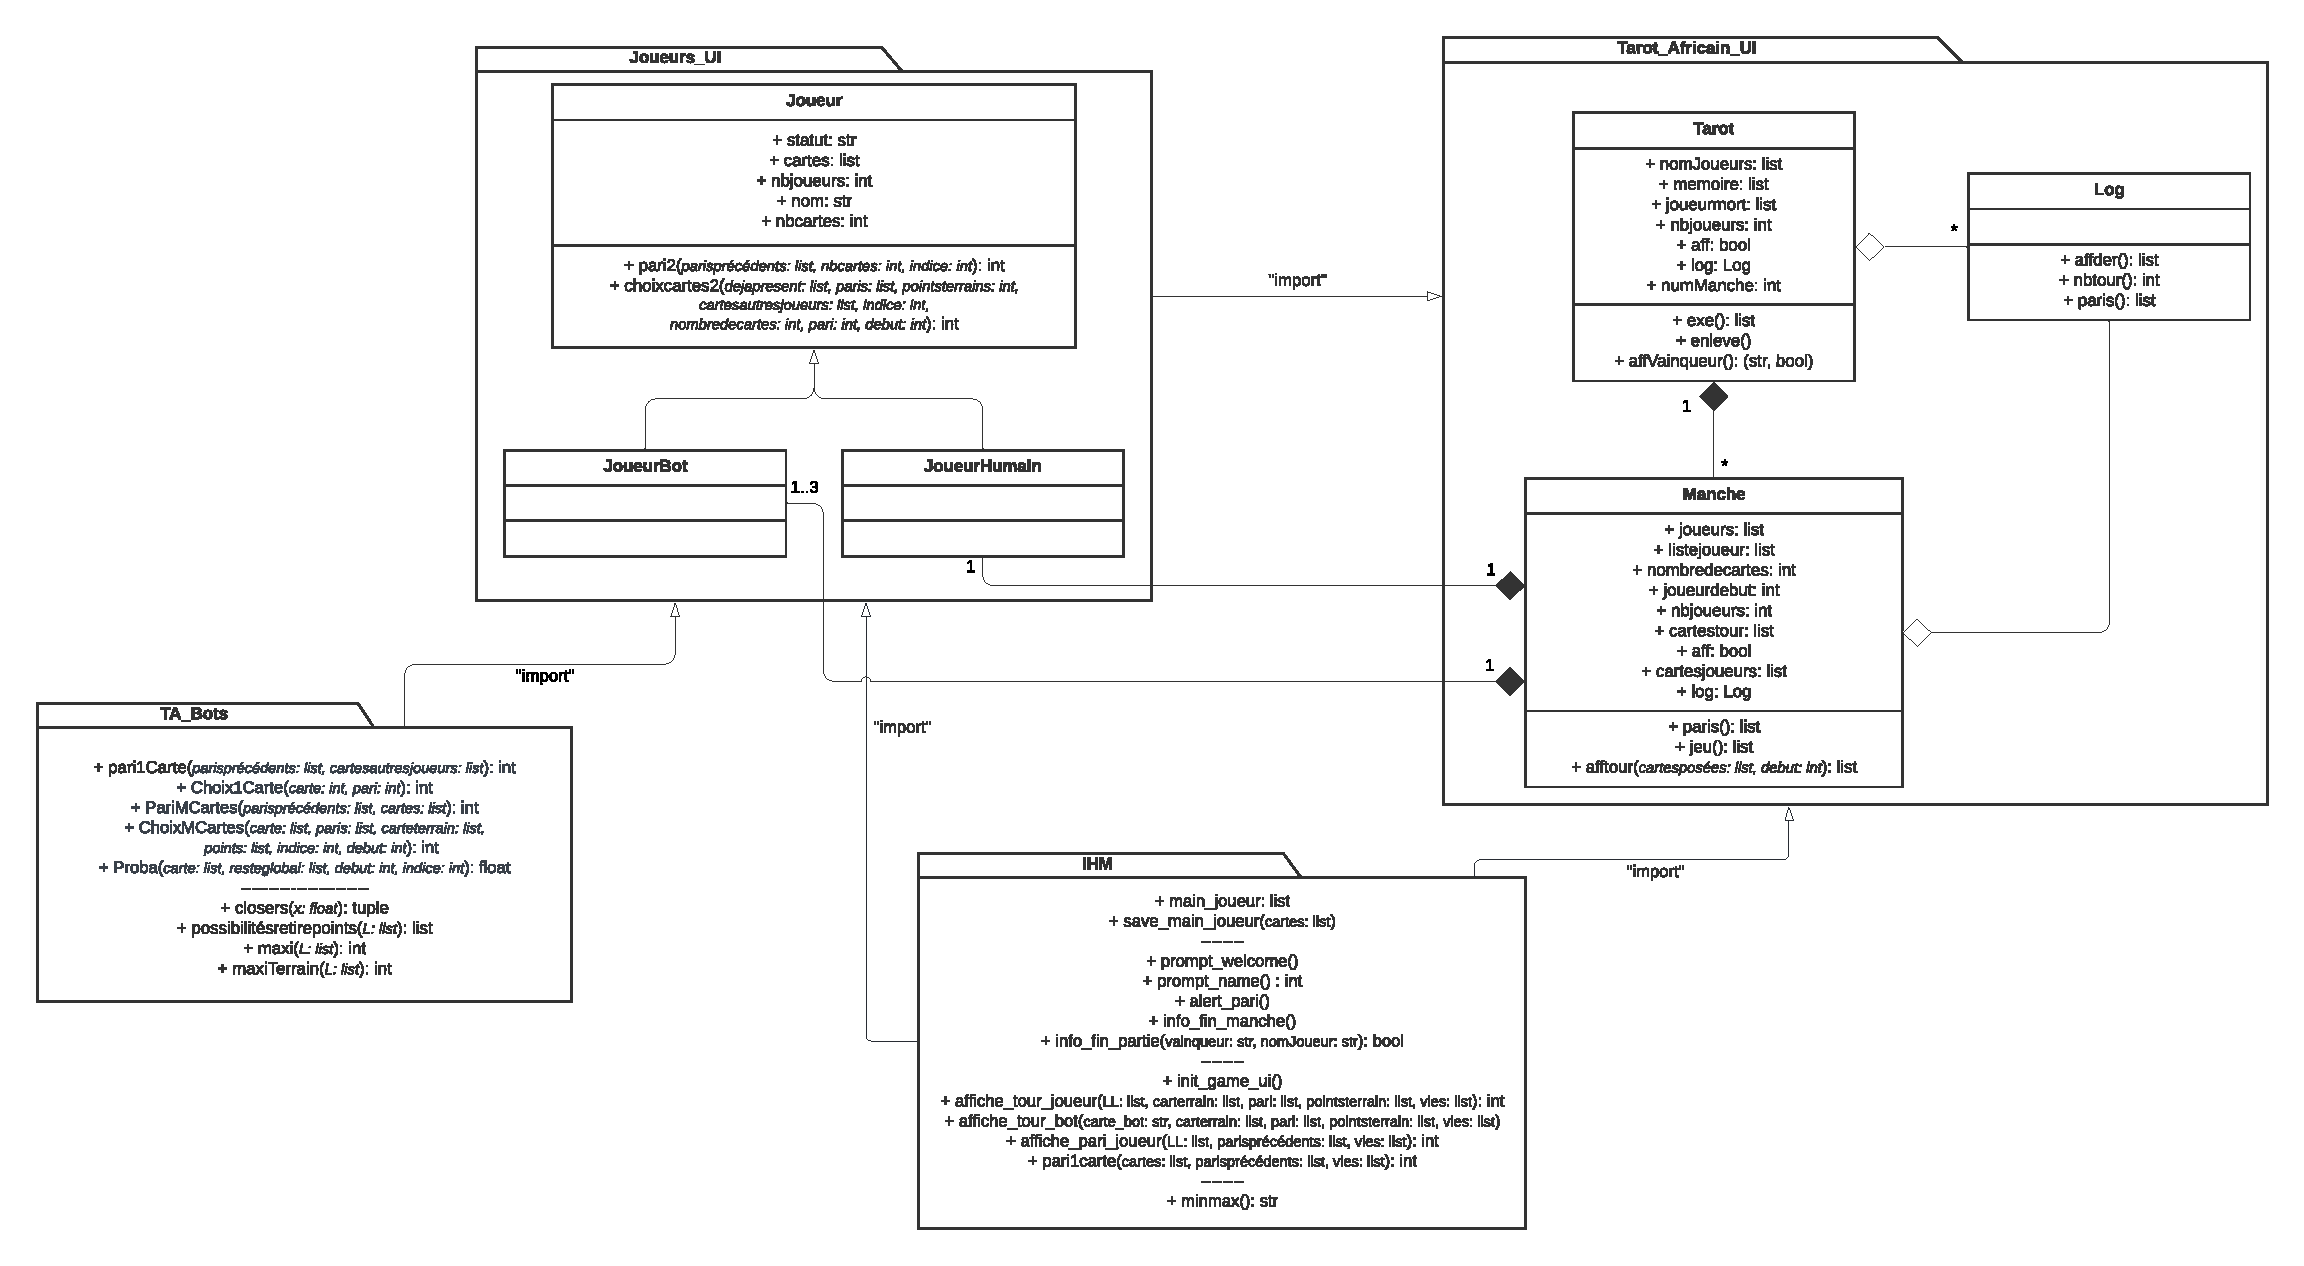
\includegraphics[height=.87\textwidth]{imgs/ClassDiagram_UI}
   \end{center}

\end{landscape}

   \begin{landscape}
   \section*{Annexe II. Fonctionnement schématique d'une partie côté \textit{backend}}
   \addcontentsline{toc}{section}{Annexe II. Fonctionnement \textit{backend} d'une partie}
   \begin{center}
      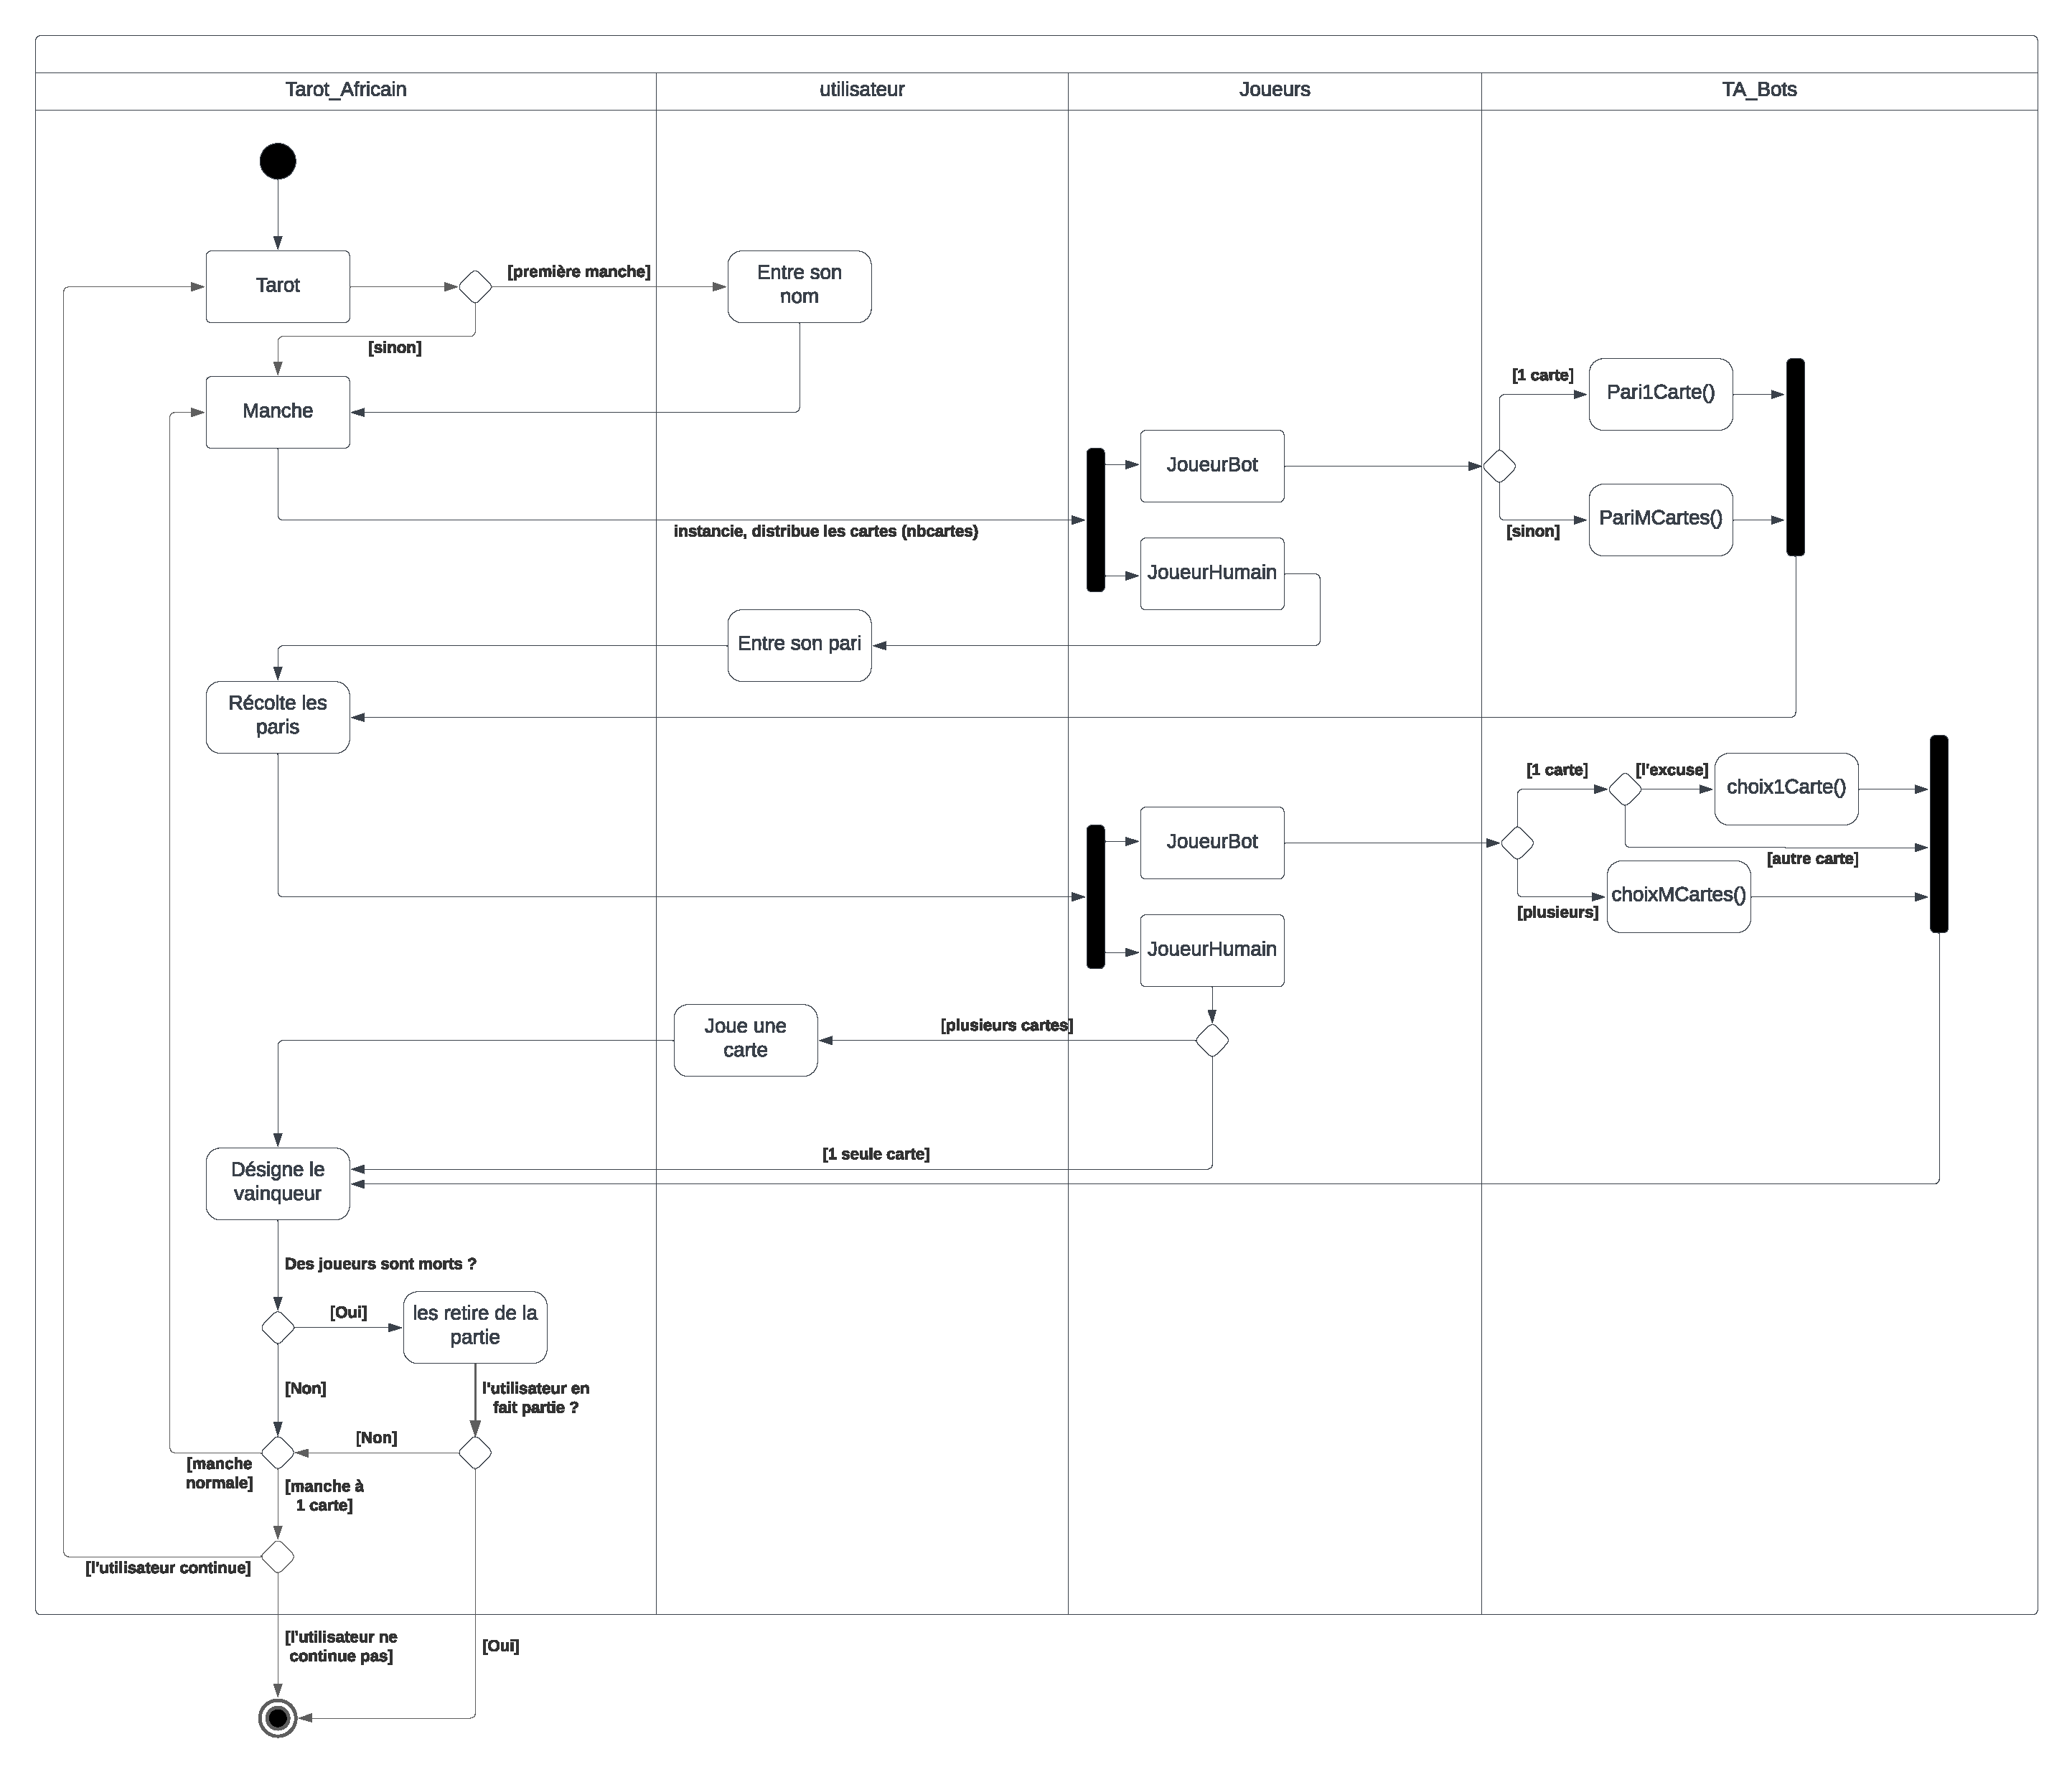
\includegraphics[height=.92\textwidth]{imgs/actDiagram}
   \end{center}
\end{landscape}


   % \section*{Conclusion}
\addcontentsline{toc}{section}{Conclusion}

   Nous avons donc pu remarquer, grâce à cette étude transversale, que les différents traceurs -- essentiels à l'amélioration et à la calibration des modèles numériques, particulièrement cruciaux à l'époque actuelle -- sont tous fortement liés entre eux.

   Une étude de l'ensemble de ces traceurs est donc nécessaire pour obtenir un réel aperçu de la situation et de l'évolution d'une partie donnée de l'océan.

%\bibliographystyle{plain}
% \bibliographystyle{ieeetr}
% \bibliography{bib/biblio}
% \addcontentsline{toc}{section}{Bibliographie}

% \listoffigures
% \addcontentsline{toc}{section}{Liste des figures}



\end{document}